%%%%% Document Setup %%%%%%%%

\documentclass[12pt, onecolumn]{revtex4}    % Font size (12pt) and column number (one or two).

\usepackage[a4paper, left=2.5cm, right=2.5cm, top=2.5cm, bottom=2.5cm]{geometry}  % Defines paper size and margin length

\renewcommand{\baselinestretch}{1}     % Defines the line spacing

\usepackage{subcaption}

\usepackage[font=small, labelfont=bf]{caption}                      % Defines caption font size and caption title bolded
\captionsetup[figure]{justification=justified, singlelinecheck=off, font=footnotesize} 
\captionsetup{compatibility=false}

\usepackage{graphics,graphicx,epsfig,ulem}	% Makes sure all graphics works
\usepackage{amsmath} 						% Adds mathematical features for equations

\usepackage{fancyhdr}

\usepackage{textcomp}

\usepackage{tabularx}

\def\thesection{\arabic{section}}
\def\thesubsection{\alph{subsection}}

\def\bibsection{\section*{References}}        % Position reference section correctly

%%%%% Document %%%%%
\begin{document}                     

\title{Testing the Milankovitch-Croll hypothesis using $\delta^{18}$O foram data} 
\maketitle
%\thispagestyle{plain} % produces page number for front page

\vspace{-4ex}

The Milankovitch-Croll hypothesis suggests that changes in the Earth's orbit around the Sun leads to changes in the Earth's planetary climate through fluctuations in solar insolation \cite{ruddiman_climate}. We can access and view this change of climate through analysing proxy data. By using deep ocean sediment cores and Earth orbital data, we can explore the hypothesis through performing various data analysis techniques and we hope to uncover whether if the theory has any validity. 

The importance of sediment cores arises from the fact that they contain a good trace for measuring the $\delta^{18}$O ratio across periods of Earth's history. The change in this ratio can provide us with an indication of how the global temperature has been fluctuating, this could then be linked to other changes on the Earth such as whether global ice volume was increasing or decreasing. \\

Defined from laboratory experiments, for a $\sim 5^{\circ}\mathrm{C}$ temperature increase there is a $\sim 1$\textperthousand\ decrease in the $\delta^{18}$O ratio of the foram shell. Looking at Figure \ref{fig:foram_data} we can see two example periods from Earth's history, a more recent and an older period. We find that in the more recent age the amplitude of the $\delta^{18}$O varies more considerably than from 4 Myr to 5 Myr, this suggests that in more recent times there have been longer periods of cooling and a more dramatic shift in temperature. Comparatively, the older $\delta^{18}$O data still has the sinusoidal-trend, suggesting that the glacial-interglacial events are a normal part of Earth's planetary climate cycle. \\

We could suggest that due to the periodic nature of the foram data, there must be a connection to the cyclical Earth-Sun orbital relationship. Through the analysis of such data we can investigate if a connection exists. We can begin by split up the phenomena into three separate but interlinked features, namely eccentricity, obliquity, and precession. \\

The eccentricity describes how elliptical the orbit is of the Earth around the Sun\cite{carroll_astro} 

\newpage

%\twocolumngrid

\bibliographystyle{unsrt}
\bibliography{practical_2}

\newpage

\section*{Appendices}
\begin{figure}[!h]
\begin{center}
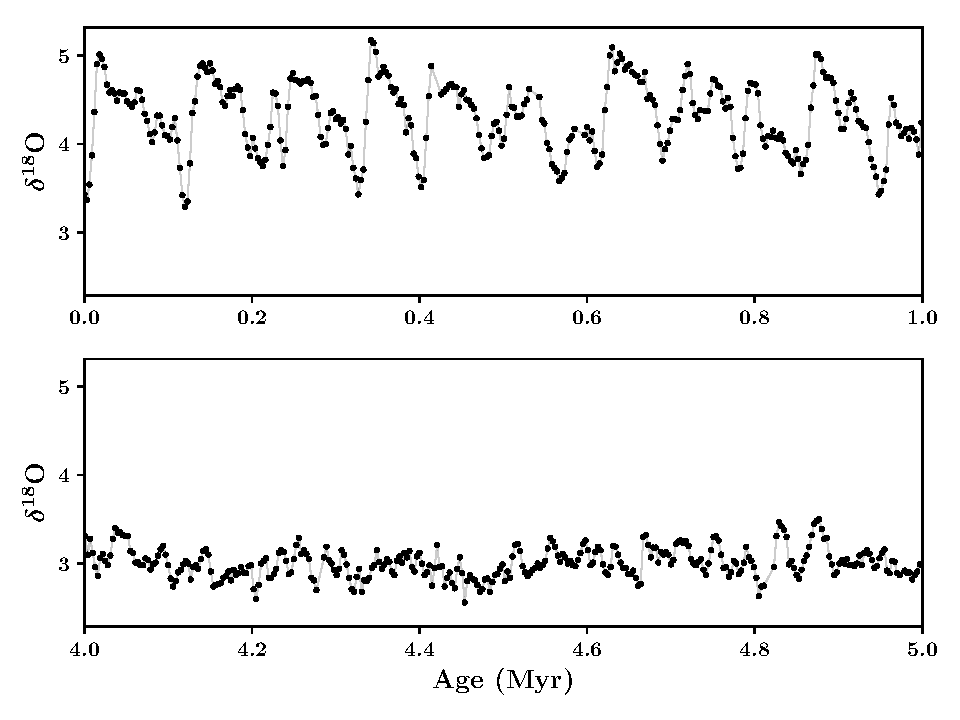
\includegraphics[width=11cm]{figures/foram_data}
\caption[]{Plots of the marine benthic foram $\delta^{18}$O data against age since the present day (the holocene). Both data sets have been taken out of a larger set which spans from 0 Myr to 6 Myr. We see that as we move closer towards the present day, the periodicity and amplitude is larger which implies that there is a more extreme temperature variation.}
\vspace{-3ex}
\label{fig:foram_data}
\end{center}
\end{figure}

\begin{figure}[!h]
\begin{center}
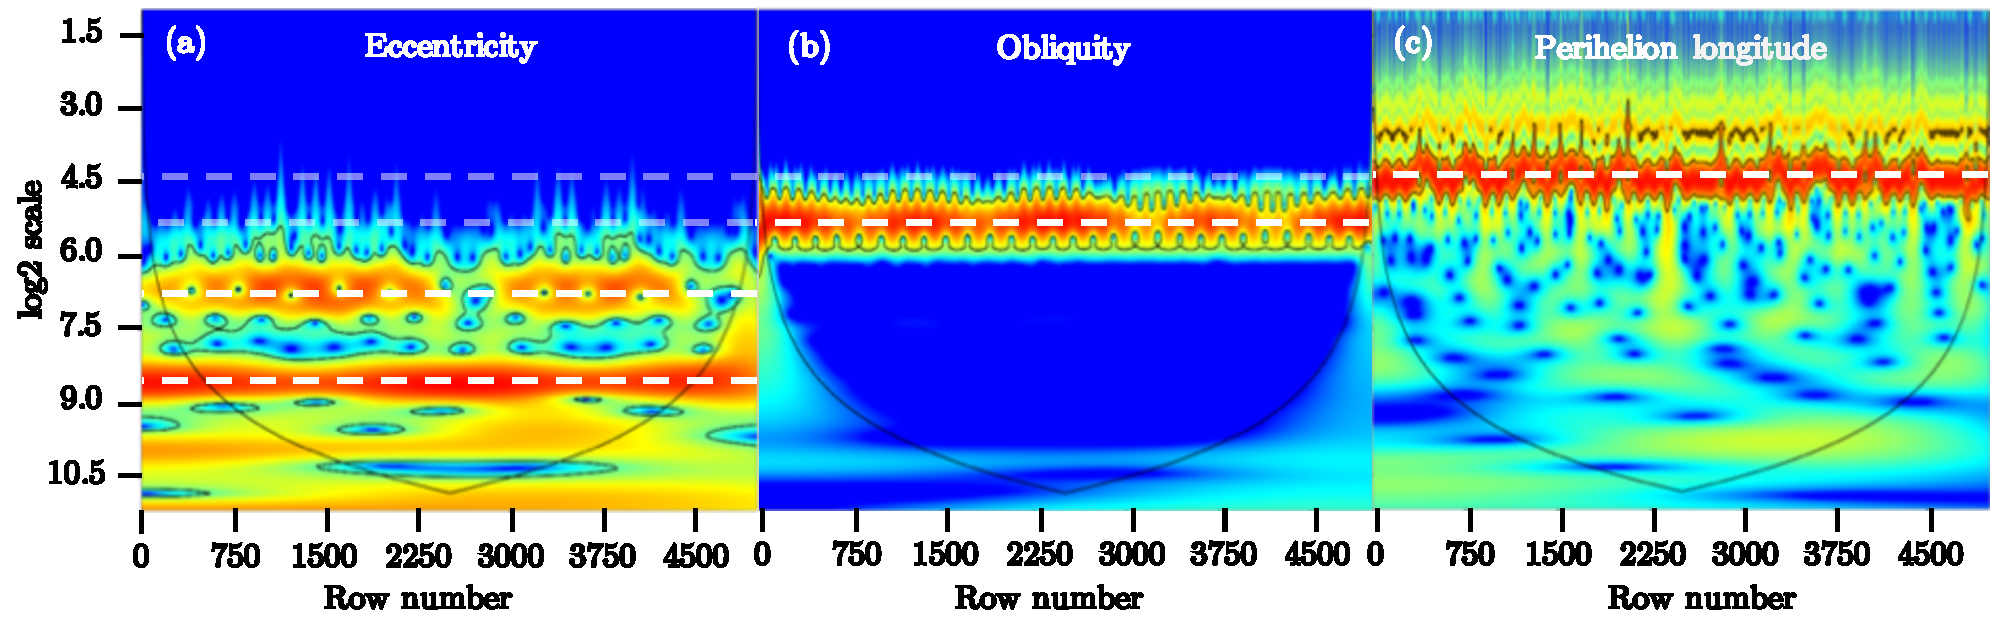
\includegraphics[width=16cm]{figures/wa_orbital_data}
\caption[]{The eccentricity, obliquity and perihelion longitude orbital data processed with the wavelet analysis tool in PAST3. The periodicities from the data can be obtained by considering the ``hottest'' areas of each of the heat maps. In Table \ref{table:final_results} we summarise the wavelengths which can be obtained from the dashed lines.}
\vspace{-3ex}
\label{fig:wa_orbital_data}
\end{center}
\end{figure}

\begin{figure}[!h]
\begin{center}
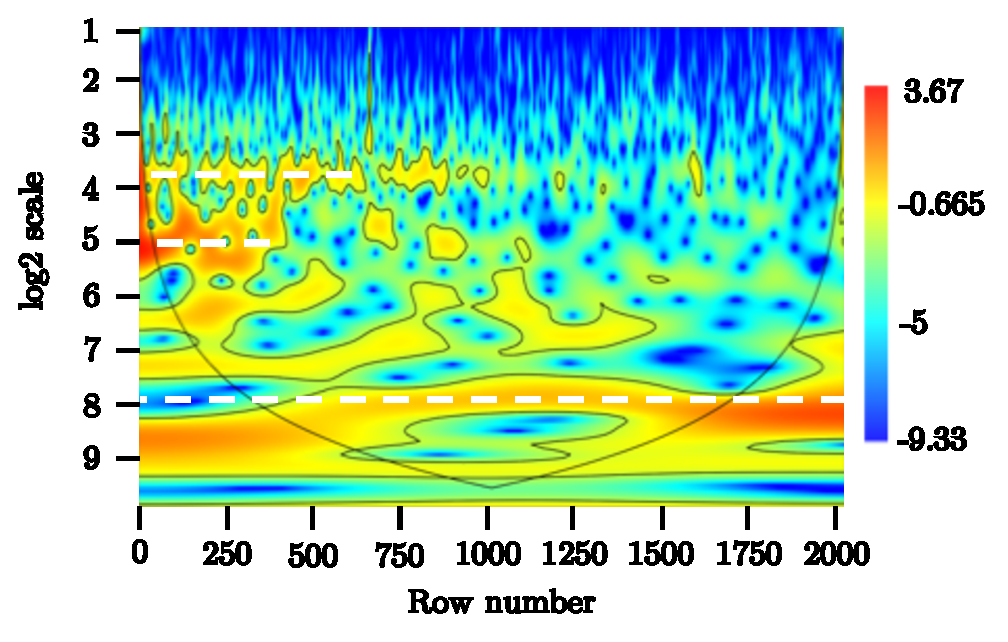
\includegraphics[width=11cm]{figures/wa_d18O.pdf}
\caption[]{Applying the PAST3 wavelet analysis tool to the $\delta^{18}$O benthic foram data we can use this as one of the possible ways to verify if the Milankovitch-Croll hypothesis is valid.}
\vspace{-3ex}
\label{fig:wa_d18o}
\end{center}
\end{figure}

\begin{figure}[!h]
\begin{center}
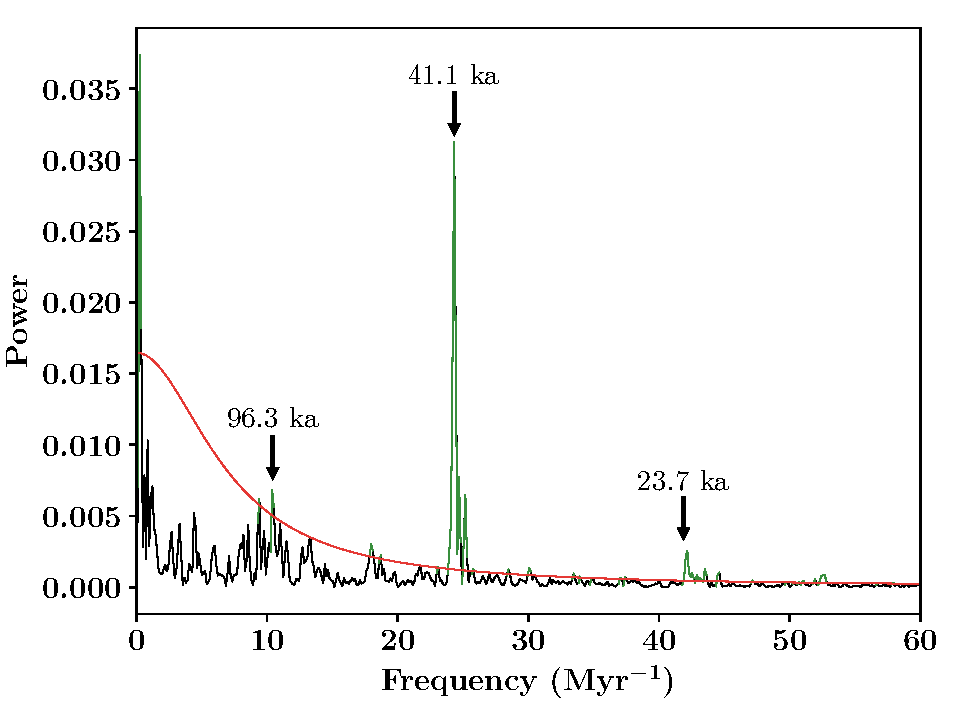
\includegraphics[width=11cm]{figures/d18O_redfit}
\caption[]{The benthic foram $\delta^{18}$O data analysed using the REDFIT spectral analysis tool in PAST3.}
\vspace{-3ex}
\label{fig:d18o_redfit}
\end{center}
\end{figure}

\begin{table}[h!]
\centering
\begin{tabular}{c@{\hskip 20pt}c@{\hskip 20pt}c} 
 \hline
  & \textbf{REDFIT Wavelengths (ka)} & \textbf{WA Wavelengths (ka)} \\ [0.5ex] 
 Eccentricity & 95.2, 128.2, 416.7 & 89.1, 100.4,  401.7\\
 Obliquity & 41.7 & 39.4 \\
 Perihelion Longitude & 23.8, 22.2 & 21.1 \\
 $\delta^{18}$O & 23.7, 41.1, 96.3  & 38.9, 96.0, 271.5, 945.5, 1247.6 \\
 \hline
\end{tabular}
\caption{The results of the REDFIT and Wavelet Analysis (WA) analysis on the orbital and benthic foram data. Provided are the wavelengths as found by using the two statistical techniques.}
\vspace{-0.5em}
\label{table:final_results}
\end{table}

\end{document}